\documentclass{article}
\usepackage{graphicx}

\title{Factorial Experiment Design}
\author{Nick Wendt}
\date{December 5, 2025}

\begin{document}
\maketitle
\section*{Basic Factorial Design}

The reason you conduct factorial experiments is to see how 
factors impact the response variable, as well as how each variable
interacts with all combinations of the other variable. This is known 
as a full factorial experiment. \\ 
  \\
However, full factorial designs can be very costly and unnecesary 
when performing experiments on many factors. Statisticians use fractional 
factorial designs during early stages of experimentation for factor selection.\\  
  \\
Sir Ronald A. Fisher wrote that coomplex designs, like factorial designs, 
are more effecient than studying each factor individually.\\
  \\
"Nature will best respond to a logical and carefully
 thought out questionnaire; indeed, if we ask her a single question, she will often refuse to answer until some other topic has been discussed."\\
   \\
Each factor will have 2 levels, high and low. 
For these notes, for some factor A, I will use $A^{+}$ for 
effect of A at high level.\\
An I will use $A^{-}$ for effect of A at low level.
\begin{itemize}
    \item Preliminary Product Process Design (PPPD) = factor screening
    \item After screening through potential inputs you can test more levels for each selected factor
    \item Need minimal experimentation
    \item Naive approach (randomly guessing) leads to way too many runs/trials
\end{itemize}

\subsection*{Steps for a Factorial Design}
\begin{enumerate}
    \item Determine the factors and levels for each factor
    \item Set up way to process experimental results
\end{enumerate}
$k = $ number of factors\\
$l = $ number of levels for each factors\\
A 2-Factorial design will require $2^{k}$ runs\\

\section*{Example}
Suppose you are a farmer and you want to improve wheat production. 
You select 2 predictors, A = water and B = sunlight, both at 2 levels, high and low.
\\
You then collect data and observe the following:
\begin{figure}[h!]
    \centering
    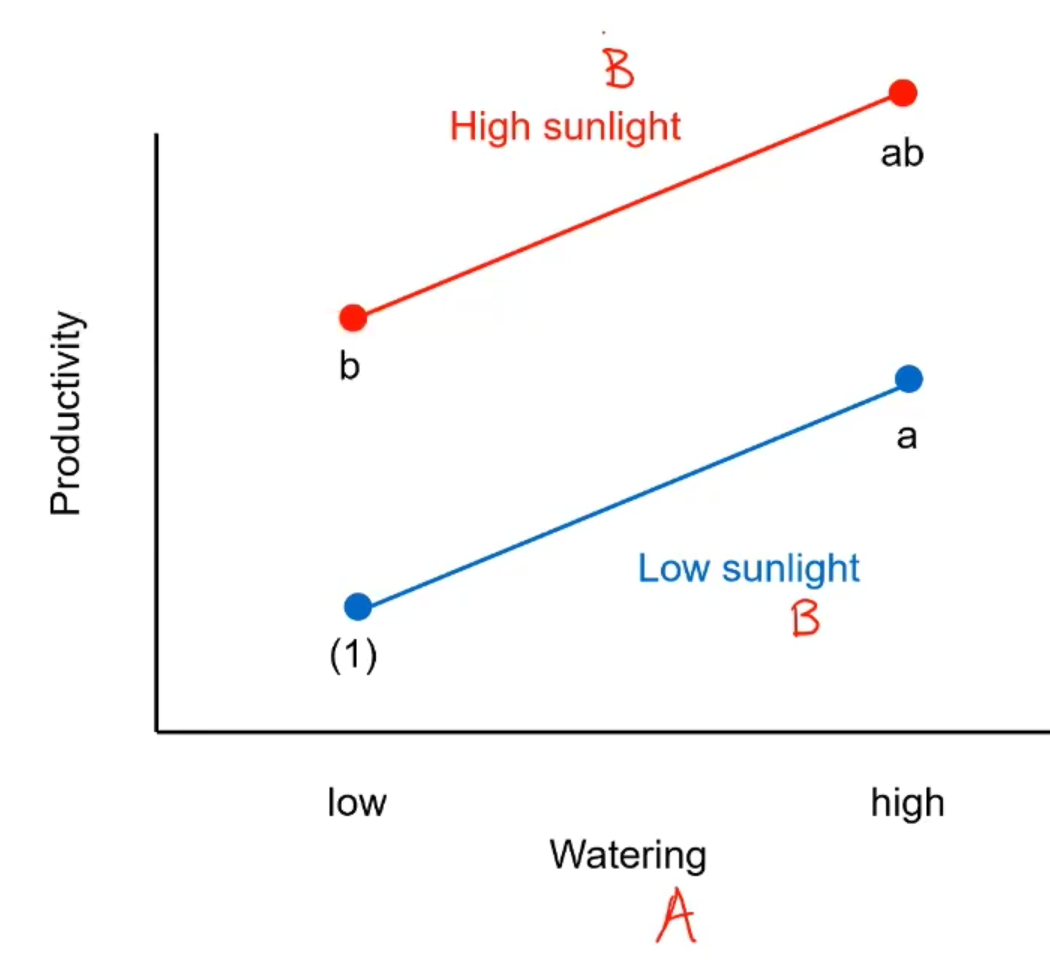
\includegraphics[width=100mm]{images/factorial2level.png}
    \caption{$2^2$ Factorial Design Example}    
\end{figure}
 


\end{document}